\documentclass{../industrial-development}
\graphicspath{{02-requirement-management/}}

\title{Управление требованиями к ПО}
\author{Антипова Наталья Андреевна, ПИ-21 МО}
\date{}

\begin{document}

\begin{frame}
  \titlepage
\end{frame}



\section{Характеристика процесса управления требованиями и его роль в промышленной разработке}
\begin{frame} \frametitle{Характеристика процесса управления требованиями}
  \begin{block}{}
	Этап \alert{«Управление требованиями»} определяется как выработка и поддержание взаимного согласия с~заказчиками по~поводу требований к~разрабатываемому ПО
  \end{block}
 	 \begin{itemize}
\item Соглашение по требованиям является связующим звеном между разработкой и управлением требованиями
\item Одобрение заказчиков "--- только половина дела, разработчики также должны принять задокументированные требования и высказаться за~создание этого продукта
  	\end{itemize}
\end{frame}



\begin{frame} \frametitle{Разделение областей разработки требований и управления ими}
 \centerline{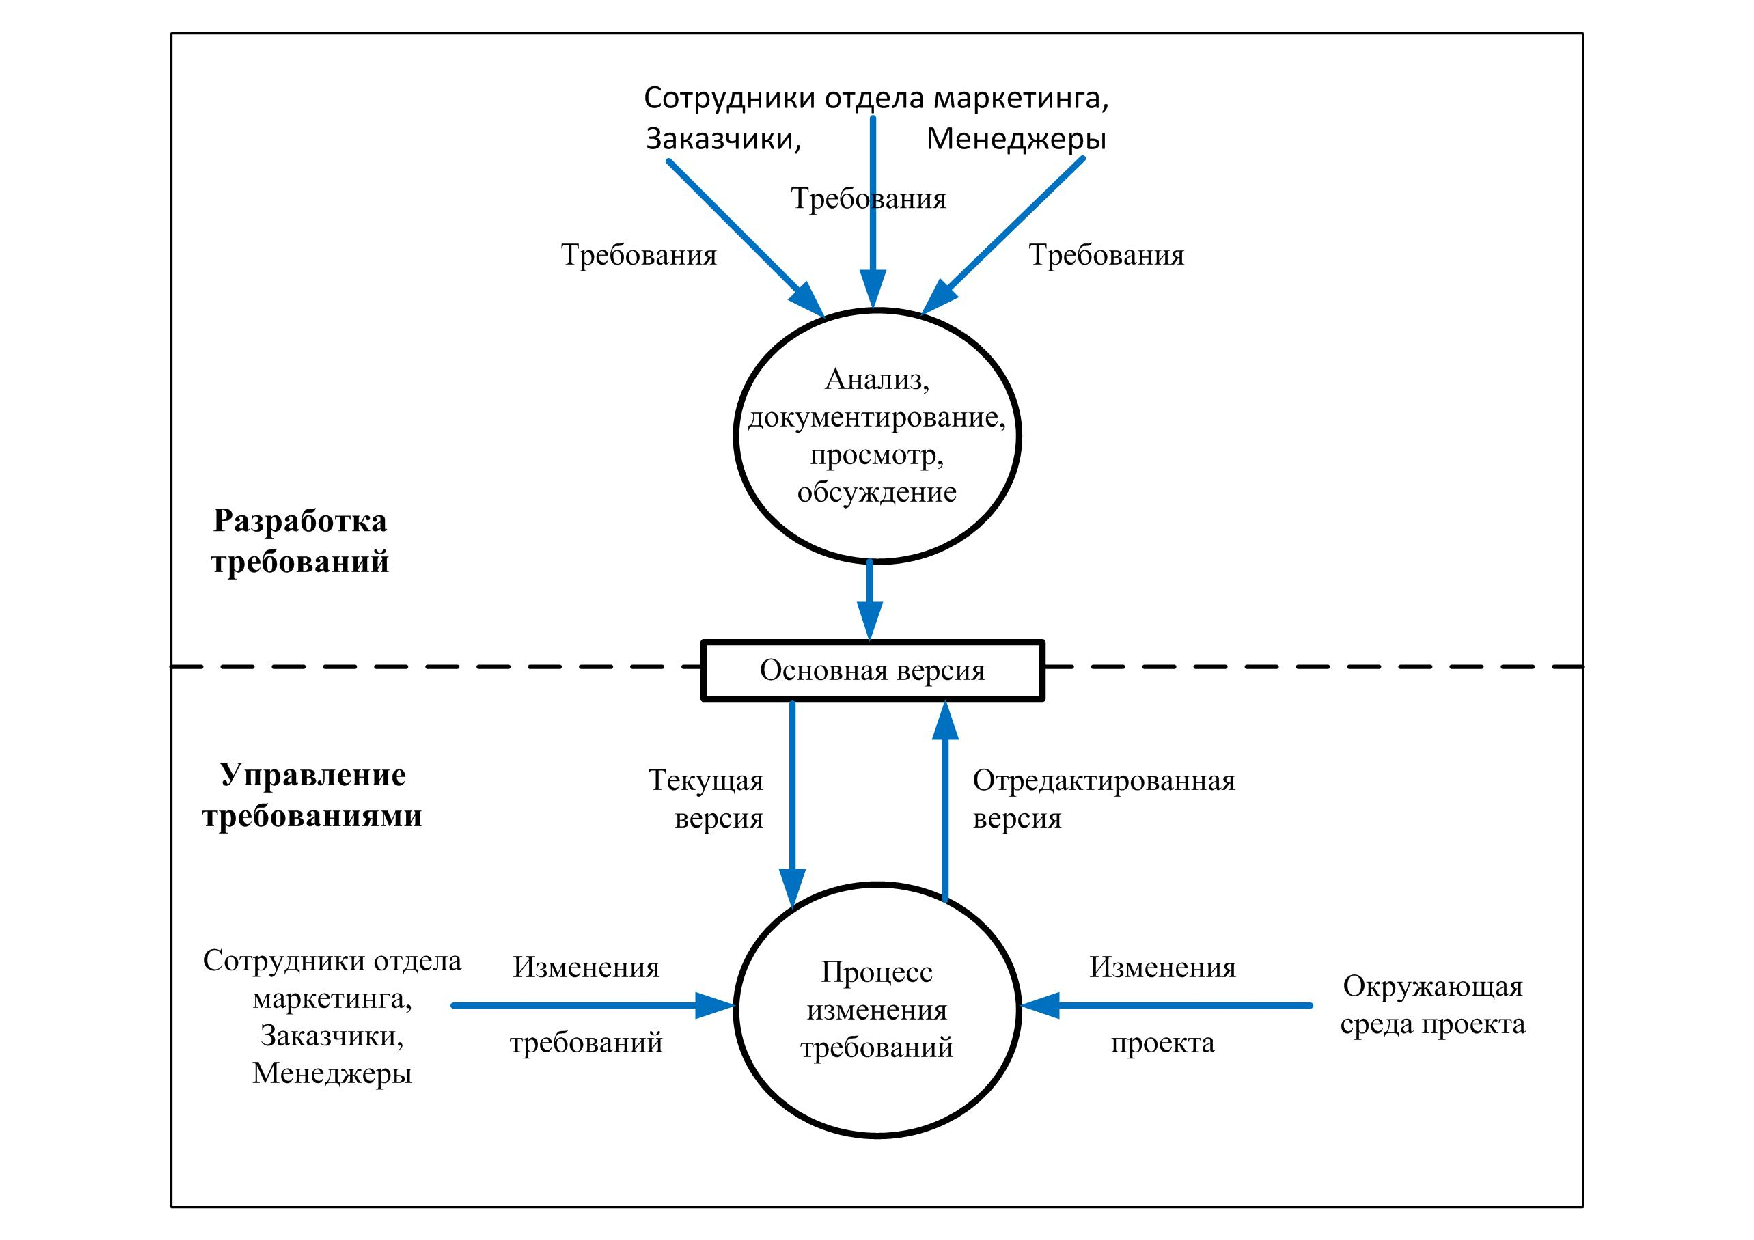
\includegraphics[width=0.9\textwidth]{pic1.pdf}}
\end{frame}

\lecturenotes

Разработку технических условий можно разделить на разработку требований и управление требованиями. 

Стадия разработки подразумевает сбор информации, анализ, уточнение и утверждение требований. Как правило, она заканчивается созданием пакета документов; документа об образе и границах продукта, документации к вариантам использования, спецификации требований к ПО, словаря данных и соответствующих моделей анализа. После проверки и одобрения этот пакет определяет базовую версию требований, соглашение между разработчиками и клиентами. Вероятно, входе разработки заключаются и дополнительные соглашения, касающиеся готового продукта, ограничений, графиков, бюджета или контрактных обязательств~\cite[с.~342]{Wiegers}. 

Начальные требования неизбежно корректируются в процессе работы заказчиками, менеджерами, специалистами по маркетингу, разработчиками и другими лицами. Для эффективного управления требованиями необходим процесс, позволяющий предлагать изменения и оценивать их возможную стоимость и влияние на проект. Решения о внесении изменений принимает совет по управлению изменениями, в который входят все заинтересованные лица. Контроль за выполнением требований на разных стадиях разработки и тестирования системы позволяет лучше понять состояние проекта в целом~\cite[с.~52--53]{Wiegers}.



\begin{frame} \frametitle{Действия по управлению требованиями}
 	 \begin{enumerate}
\item Определение основной версии требований 
\item Просмотр предлагаемых изменений требований и~оценка вероятности воздействия каждого изменения до его принятия
\item Включение одобренных изменений требований в~проект установленным способом
\item Согласование плана проекта с требованиями
\item Обсуждение новых обязательств, основанных на~оцененном влиянии изменения требований
\item Отслеживание отдельных требований до их дизайна, исходного кода и вариантов тестирования
\item Отслеживание статуса требований и~действий по~изменению на протяжении всего проекта
  	\end{enumerate}
\end{frame}



\section{Цикл работы с требованиями}
\begin{frame} \frametitle{Цикл работы с требованиями}
	\begin{enumerate}
\item Определение процесса управления изменениями
\item Создание совета по управлению изменениями
\item Анализ влияния изменений требований
\item Создание базовой версии и управление версиями требований
\item Ведение журнала изменений требований
\item Контроль за состоянием всех требований
\item Оценка изменяемости требований
\item Использование средств управления требованиями
\item Создание матрицы связей требований
	\end{enumerate}
\end{frame}



\begin{frame} \frametitle{Цикл работы с требованиями}
	1. Определение процесса управления изменениями
	\begin{itemize}
\item Определяется процесс представления, анализа и~утверждения или отклонения изменений
\item В дальнейшем этот процесс применяется для управления всеми предлагаемыми изменениями
	\end{itemize}
	2. Создание совета по управлению изменениями
	\begin{itemize}
\item Совет получает и оценивает информацию о~предполагаемых изменениях требований
\item Принятие решений об одобрении или отклонении изменений и в какой версии продукта будет внедрена та или иная функция 
	\end{itemize}
\end{frame}

\lecturenotes

1. Определяется процесс представления, анализа и утверждения или отклонения изменений. В дальнейшем этот процесс применяется для управления всеми предлагаемыми изменениями. В контексте процесса управления изменениями полезно использовать коммерческие средства отслеживания недостатков

2. Из представителей заинтересованных в проекте лиц создается совет по управлению изменениями, который будет получать информацию о предполагаемых изменениях требований, а также оценивать ее, решать, какие изменения принять, а какие отклонить, и определять, в какой версии продукта будет внедрена та или иная функция



\begin{frame} \frametitle{Цикл работы с требованиями}
	3. Анализ влияния изменений требований
	\begin{itemize}
\item Оценивается, как каждое предлагаемое изменение требований повлияет на проект
\item Определяется, что необходимо для реализации изменений
\item Оцениваются затраты на реализацию
	\end{itemize} 
	4. Создание базовой версии и управление версиями требований
	\begin{itemize}
\item Базовая версия содержит требования, утвержденные для реализации в конкретной версии продукта 
\item Всем версиям спецификации требований присваиваются уникальные идентификаторы
	\end{itemize}
\end{frame}

\lecturenotes

3. Анализ влияния изменений помогает совету по управлению изменениями принимать обоснованные решения. Оценивается, как каждое предлагаемое изменение требований повлияет на проект. На основе матрицы связей выявляются другие требования, элементы архитектуры, исходный код и сценарии тестирования, которые, возможно, придется изменить. Также определяется, что необходимо для реализации изменений, и оцениваются затраты на реализацию

4. Базовая версия содержит требования, утвержденные для реализации в конкретной версии продукта. После определения базовых требований изменения можно вносить только в соответствии с процессом управления изменениями. Всем версиям спецификации требований присваиваются уникальные идентификаторы, чтобы избежать путаницы между черновыми вариантами и базовыми версиями, а также между предыдущей и текущей версиями требований. Более надежное решение "--- управлять версиями документов с требованиями при помощи соответствующих средств управления конфигурацией.


\begin{frame} \frametitle{Цикл работы с требованиями}
	5. Ведение журнала изменений требований
	\begin{itemize}
\item Фиксируются даты изменения спецификаций требований, сами коррективы и их причины
\item Указываются лица, вносившие изменения
	\end{itemize} 
	6. Контроль за состоянием всех требований
	\begin{itemize}
\item Создается БД, включающая по одной записи для~каждого требования
\item В БД заносятся ключевые атрибуты каждого требования, включая его состояние
	\end{itemize} 
\end{frame}

\lecturenotes

5. Фиксируются даты изменения спецификаций требований, сами коррективы и их причины, а также указываются лица, вносившие изменения. Автоматизировать эти задачи позволяет утилита управления версиями или коммерческая утилита управления требованиями.

6. Создается БД, включающая по одной записи для каждого дискретного функционального требования. В БД заносятся ключевые атрибуты каждого требования, включая его состояние (например «предложено», «одобрено», «реализовано» или «проверено»), чтобы в любой момент можно было узнать количество требований в каждом состоянии



\begin{frame} \frametitle{Цикл работы с требованиями}
	7. Оценка изменяемости требований
	\begin{itemize}
\item Еженедельно фиксируется количество требований, внесенных в базовую версию, а~также число предложенных и одобренных изменений
\item Если требования формируются не самим клиентом, а~от~его лица, может оказаться, что проблема понята плохо
	\end{itemize} 
	8. Использование средств управления требованиями
	\begin{itemize}
\item Коммерческие утилиты управления требованиями позволяют хранить различные типы требований в БД 
\item Для каждого требования можно определить атрибуты, отследить его состояние, а также выявить связи между требованиями и другими рабочими продуктами
	\end{itemize} 
\end{frame}

\lecturenotes

7. Еженедельно фиксируется количество требований, внесенных в базовую версию, а также число предложенных и одобренных изменений (добавлений, модификаций и удалений). Если требования формируются не самим клиентом, а от его лица, может оказаться, что проблема понята плохо, границы проекта определены нечетко, при сборе информации многие требования были упущены или внутрикорпоративные политики меняются в худшую сторону.

8. Коммерческие утилиты управления требованиями позволяют хранить различные типы требований в БД. Для каждого требования можно определить атрибуты, отслеживать его состояние, а также выявить связи между требованиями и другими рабочими продуктами. Данный прием помогает автоматизировать многие задачи по управлению требованиями.



\begin{frame} \frametitle{Цикл работы с требованиями}
	9. Создание матрицы связей требований
	\begin{itemize}
\item Создается таблица, сопоставляющая все функциональные требования с элементами архитектуры, кода и тестами
\item Матрица связей требований позволяет сопоставить функциональные требования с требованиями более высоких уровней и с другими родственными требованиями
	\end{itemize}
\end{frame}

\lecturenotes

9. Создается таблица, сопоставляющая все функциональные требования с элементами архитектуры и кода, которые реализуют данное требование, и с тестами, проверяющими его. Матрица связей требований позволяет также сопоставить функциональные требования с требованиями более высоких уровней, на основе которых они созданы, и с другими родственными требованиями. Заполняется эта таблица в ходе, а не в конце работы над проектом



\section{Принципы и приемы управления требованиями}
\begin{frame} \frametitle{Базовая версия требований}
  \begin{block}{}
	\alert{Базовая версия} "--- это набор функциональных и~нефункциональных требований, которые разработчики обязались реализовать в определенной версии
  \end{block}	
	\begin{itemize}
\item Чтобы договориться об изменении требований, сначала нужно их зафиксировать в «первозданном виде»
\item Определение базовой версии позволяет выработать общее понимание возможностей и свойств, которые необходимы в данной версии
\item Последующие изменения разрешается вносить только через~определенный в проекте процесс управления изменениями
  	\end{itemize}
\end{frame}

\lecturenotes

\textbf{Базовая версия} "--- это набор функциональных и нефункциональных требований, которые разработчики обязались реализовать в определенной (выбранной) версии. Определение базовой версии позволяет заинтересованным в проекте лицам выработать общее понимание возможностей и свойств, которые они хотят видеть в данной версии. Принятая базовая версия требований, как правило, становится базовой после официальных экспертизы и утверждения. Последующие изменения разрешается вносить в нее только через определенный в проекте процесс управления изменениями. До принятия базовой версии требования все еще изменяются, поэтому не имеет смысла ограничивать модификацию какими-то процедурами. Однако необходимо начинать контролировать версии, уникальным образом идентифицируя разные версии каждого документа требований, сразу после того, как сделан предварительный набросок этого документа~\cite[с.~344]{Wiegers}. 

Соглашение по требованиям является связующим звеном между разработкой и управлением требованиями. У членов команды должен быть доступ к текущим требованиям на протяжении всего проекта, возможно, через Web-решения посредством инструментов управления требованиями~\cite[с.~342]{Wiegers}. 



\begin{frame} \frametitle{Процедура управления требованиями (1)}
базируется на:
	\begin{itemize}
\item инструментах, приемах и соглашениях по управлению версиями различных документов требований и~отдельных требований
\item правилах составления базовой версии требований
\item статусах требований, которые будут использоваться, и~категориях лиц, которые имеют право изменять их
\item процедурах контроля за статусом требования
  	\end{itemize}
\end{frame}

\begin{frame} \frametitle{Процедура управления требованиями (2)}
	\begin{itemize}
\item способах, с помощью которых новые требования и~изменения существующих требований предлагаются, обрабатываются, обсуждаются и~передаются всем заинтересованным лицам
\item методах анализа влияния предложенного изменения
\item отслеживании связей планов и обязательств проекта с~изменением требований
  	\end{itemize}
\end{frame}

\lecturenotes

Всю эту информацию можно включить в одно описание процесса управления требованиями. Или же разработать отдельные процедуры для контроля за изменениями, анализа влияния и контроля за состоянием. Эти процедуры следует довести до сведения каждого сотрудника организации, поскольку они представляют общие функции, которые должны выполняться каждым проектной командой.

Кто-то должен выполнять действия при управлении требованиями, поэтому в описаниях процесса также следует определить роли участников, ответственных за выполнение каждой задачи. Проектный аналитик требований, как правило, несет основную ответственность за управление требованиями. Он выбирает механизм сохранения требований (например, средство управления требованиями), определяет атрибуты требований, скоординирует обновление данных о состоянии и отслеживаемости требований и сгенерирует отчеты об изменении действий~\cite[с.~345]{Wiegers}.

Управление требованиями – это рабочий процесс, следовательно, он должен подчиняться определённым правилам и процедурам~\cite[с.~72]{Maglinec}.



\begin{frame} \frametitle{Контроль статуса требований (1)}
\begin{tabular}{|p{2,4cm}|p{7,6cm}|}
	\hline \textbf{Состояние} & \textbf{Определение} \\
	\hline Предложено (Proposed) & Требование запрошено авторизированным источником\\
	\hline Одобрено (Approved) & Требование проанализировано, его влияние на проект просчитано, и оно было размещено в базовой версии определенной версии. Ключевые заинтересованные в проекте лица согласились с этим требованием, а разработчики ПО обязались реализовать его\\
	\hline Реализовано (Implemented) & Код, реализующий требование, разработан, написан и протестирован. Требование отслежено до соответствующих элементов дизайна и кода \\
	\hline 
\end{tabular}
\end{frame}

\lecturenotes

В автоматизированных средствах управления проектами для контроля степени выполнения той или иной работы используется понятие степени выполнения, выражаемой в процентах. Данный способ слабо применим в программистских разработках, где, в силу их слабой формализованности, трудно оценить работу в процентах. При управлении требованиями рекомендуется оперировать не процентом, а статусом. 

Контроль статуса каждого функционального требования на протяжении всей разработки позволяет более точно оценивать готовность проекта. В таблице перечислено несколько возможных состояний требований~\cite[с.~74]{Maglinec}.



\begin{frame} \frametitle{Контроль статуса требований (2)}
\begin{tabular}{|p{2,4cm}|p{7,6cm}|}
	\hline \textbf{Состояние} & \textbf{Определение} \\
	\hline Проверено (Verified) & Корректное функционирование реализованного требования подтверждено в~соответствующем продукте. Требование отслежено до соответствующих вариантов тестирования. Теперь требование считается завершенным\\
	\hline Удалено (Deleted) & Утвержденное требование удалено из базовой версии. Опишите причины удаления и назовите того, кто принял это решение\\
	\hline Отклонено (Rejected) & Требование предложено, но не запланировано для реализации ни в одной будущих версий. Опишите причины отклонения требования и назовите того, кто принял это решение\\
	\hline 
\end{tabular}
\end{frame}



\begin{frame} \frametitle{Основные трудозатраты по управлению требованиями}
	\begin{itemize}
\item предложение изменения требований и новых требований
\item оценка предложенных изменений, включая оценку влияния изменения
\item изменение работы
\item обновление документации требований или базы данных
\item сообщение об изменениях требований заинтересованным группам и отдельным лицам
\item контроль и отчет о состоянии требования
\item сбор информации об отслеживаемости требований
  	\end{itemize}
\end{frame}

\lecturenotes

Для измерения непосредственных усилий на разработку и управление проектом необходимо заняться корпоративной культурой и дисциплиной сотрудников "--- только так удастся фиксировать ежедневную работу. На это уходит не так много времени, как многие считают. Команда сможет получить ценные идеи, поняв, как на самом деле тратятся усилия на различные задачи проекта.

Контроль усилий также позволяет выяснить, выполняют ли разработчики предполагаемые задачи для управления требованиями. Неудача в управлении требований увеличивает риск появления неуправляемых изменений и требований, по неосторожности пропущенных к ходе реализации~\cite[с.~354]{Wiegers}.



\begin{frame} \frametitle{Незапланированные изменения}
  \begin{block}{}
Незапланированным изменением требований считается предложение новой функциональности и~существенной модификации после утверждения базовой версии требований к проекту
  \end{block}
	\begin{itemize}
\item Проблема заключается не в изменении требований, а~в~том, что запоздалые изменения оказывают существенное влияние на уже проделанную работу
\item Ключевая стратегия ограничения роста незапланированных требований "--- разработка хороших требований в максимальном контакте с~заказчиком
\item Другая стратегия "--- это умение сказать: «Нет». Обычно «Нет» заменяется на «Не сейчас»
  	\end{itemize}
\end{frame}

\lecturenotes

Незапланированным изменением требований считается предложение новой функциональности и существенной модификации после утверждения базовой версии требований к проекту. Чем дольше продолжается работа над проектами, тем больше их объем.
	\begin{itemize}
\item Проблема заключается не в изменении требований, а в том, что запоздалые изменения оказывают существенное влияние на уже проделанную работу. Если каждый запрос на изменение будет удовлетворяться "--- проект, возможно, никогда не будет завершён.
\item Ключевая стратегия ограничения роста незапланированных требований "--- разработка хороших требований в максимальном контакте с заказчиком.
\item Другая стратегия – это умение сказать: «Нет». Обычно предлагается «смягчить» этот подход, заменив «Нет», на «Не сейчас» (требование обязательно будет выполнено, но не в текущей версии). Опыт показывает, что данная фраза значительно упрощает общение и позволяет сподвигнуть представителя Заказчика на размышления: а действительно ли его идея хороша, а какую конкретную пользу она принесёт бизнесу его предприятия?
  	\end{itemize}
Не следует делать вывод, что изменения не нужны. Изменения неизбежны, приемлемы и в ряде случаев благоприятны. Бизнес-процессы, рыночные возможности, конкурирующие продукты, и технологии "--- все они могут меняться в ходе разработки продукта, и менеджеры могут определить, как в ответ на эти изменения необходимо откорректировать направление работы\cite[с.~359]{Wiegers}.



\begin{frame} \frametitle{Процесс контроля изменений}
позволяет:
	\begin{itemize}
\item контролировать затраты на жизненный цикл продукта
\item отслеживать статус всех предложенных изменений
\item гарантировать отсутствие пропусков и потерь требований
\item руководителю проекта принимать обоснованные бизнес-решения
  	\end{itemize}
Процесс контроля изменений должен быть тщательно задокументирован, максимально прост и, что важнее всего, эффективен. 
\end{frame}

\lecturenotes

После регистрации запроса на изменение необходимо принять решение о его дальнейшей судьбе. Совет по управлению изменениями (change control board, CCB) (иногда его называют советом по управлению конфигурацией) был признан лучшим практическим решением при разработке ПО. На практике функции Совета могут быть делегированы и одному человеку (в зависимости от размеров проекта).

Запрос на изменение может быть принят, либо отклонён. В первом случае его необходимо включить в план работ над проектом, во втором "--- сформулировать мотивированный отказ. При принятии решения по запросу необходимо исходить: а) из степени важности запроса для Заказчика и б) из его стоимости для Разработчика. Стоимость определяется на основании анализа влияния изменения~\cite[с.~75--76]{Maglinec}.



\begin{frame} \frametitle{Анализ влияния изменения}
Анализ влияния обеспечивает точное понимание подтекста предложенного изменения, что помогает команде принимать информированные бизнес-решения о~том, какое изменение одобрить

\setlength\parindent{0.5cm}Анализ затрагивает три аспекта:
	\begin{enumerate}
\item Определение возможных последствий изменения
\item Определение всех файлов, моделей и документов, которые придется изменить в случае принятия изменения
\item Определение задач, необходимых для реализации изменения, и оценка усилий, необходимых для~выполнения этих задач
  	\end{enumerate}
\end{frame}

\lecturenotes

Анализ влияния обеспечивает точное понимание подтекста предложенного изменения, что помогает команде принимать информированные бизнес-решения о том, какое изменение одобрить. Анализ позволяет выявить компоненты, которые возможно понадобиться создать, изменить или отклонить, и оценить затраты, связанные с реализацией изменения. До того, как разработчик ответит: «Конечно, без проблем», он должен потратить время на анализ результата изменения.

Председатель совета по управлению изменениями обычно просит опытного разработчика выполнить анализ результата.

Анализа результатов изменений затрагивает три аспекта:
	\begin{enumerate}
\item Определение возможных последствий изменения. Часто они вызывают значительный волновой эффект. Включение множества функций в продукт может снизить его производительность до неприемлемого уровня.
\item Определение всех файлов, моделей и документов, которые придется изменить в случае принятия изменения
\item Определение задач, необходимых для реализации изменения, и оценка усилий, необходимых для выполнения этих задач
  	\end{enumerate}




\begin{frame} \frametitle{Отслеживаемость требований}
  \begin{block}{}
Отслеживаемость требований документирует зависимости и~логические связи отдельных требований и~других элементов системы
  \end{block}
	\begin{itemize}
\item Связи отслеживаемости помогают следить за развитием требования в обоих направлениях "--- от~первоисточника к~реализации и наоборот 
\item Отслеживаемость позволяет отслеживать родительские требования, взаимосвязи и зависимости между отдельными требованиями
\item Информация о связях отслеживаемости показывает влияние изменения, если отдельное требование удаляется или модифицируется
  	\end{itemize}
\end{frame}

\lecturenotes

Отслеживаемость требований документирует зависимости и логические связи отдельных требований и других элементов системы (архитектуры, модулей исходного кода, требований различных типов и др.)
	\begin{itemize}
\item Связи отслеживаемости помогают следить за развитием требования в обоих направлениях "--- от~первоисточника к~реализации и наоборот 
\item Отслеживаемость позволяет отслеживать родительские требования, взаимосвязи и зависимости между отдельными требованиями
\item Информация о связях отслеживаемости показывает влияние изменения, если отдельное требование удаляется или модифицируется
  	\end{itemize}
Отслеживаемость представляет собой одну из качеств хороших требований. Для осуществления анализа отслеживаемости каждое требование должно быть уникально идентифицировано~\cite[с.~77]{Maglinec}


\begin{frame} \frametitle{Четыре типа отслеживаемости требований }
 \centerline{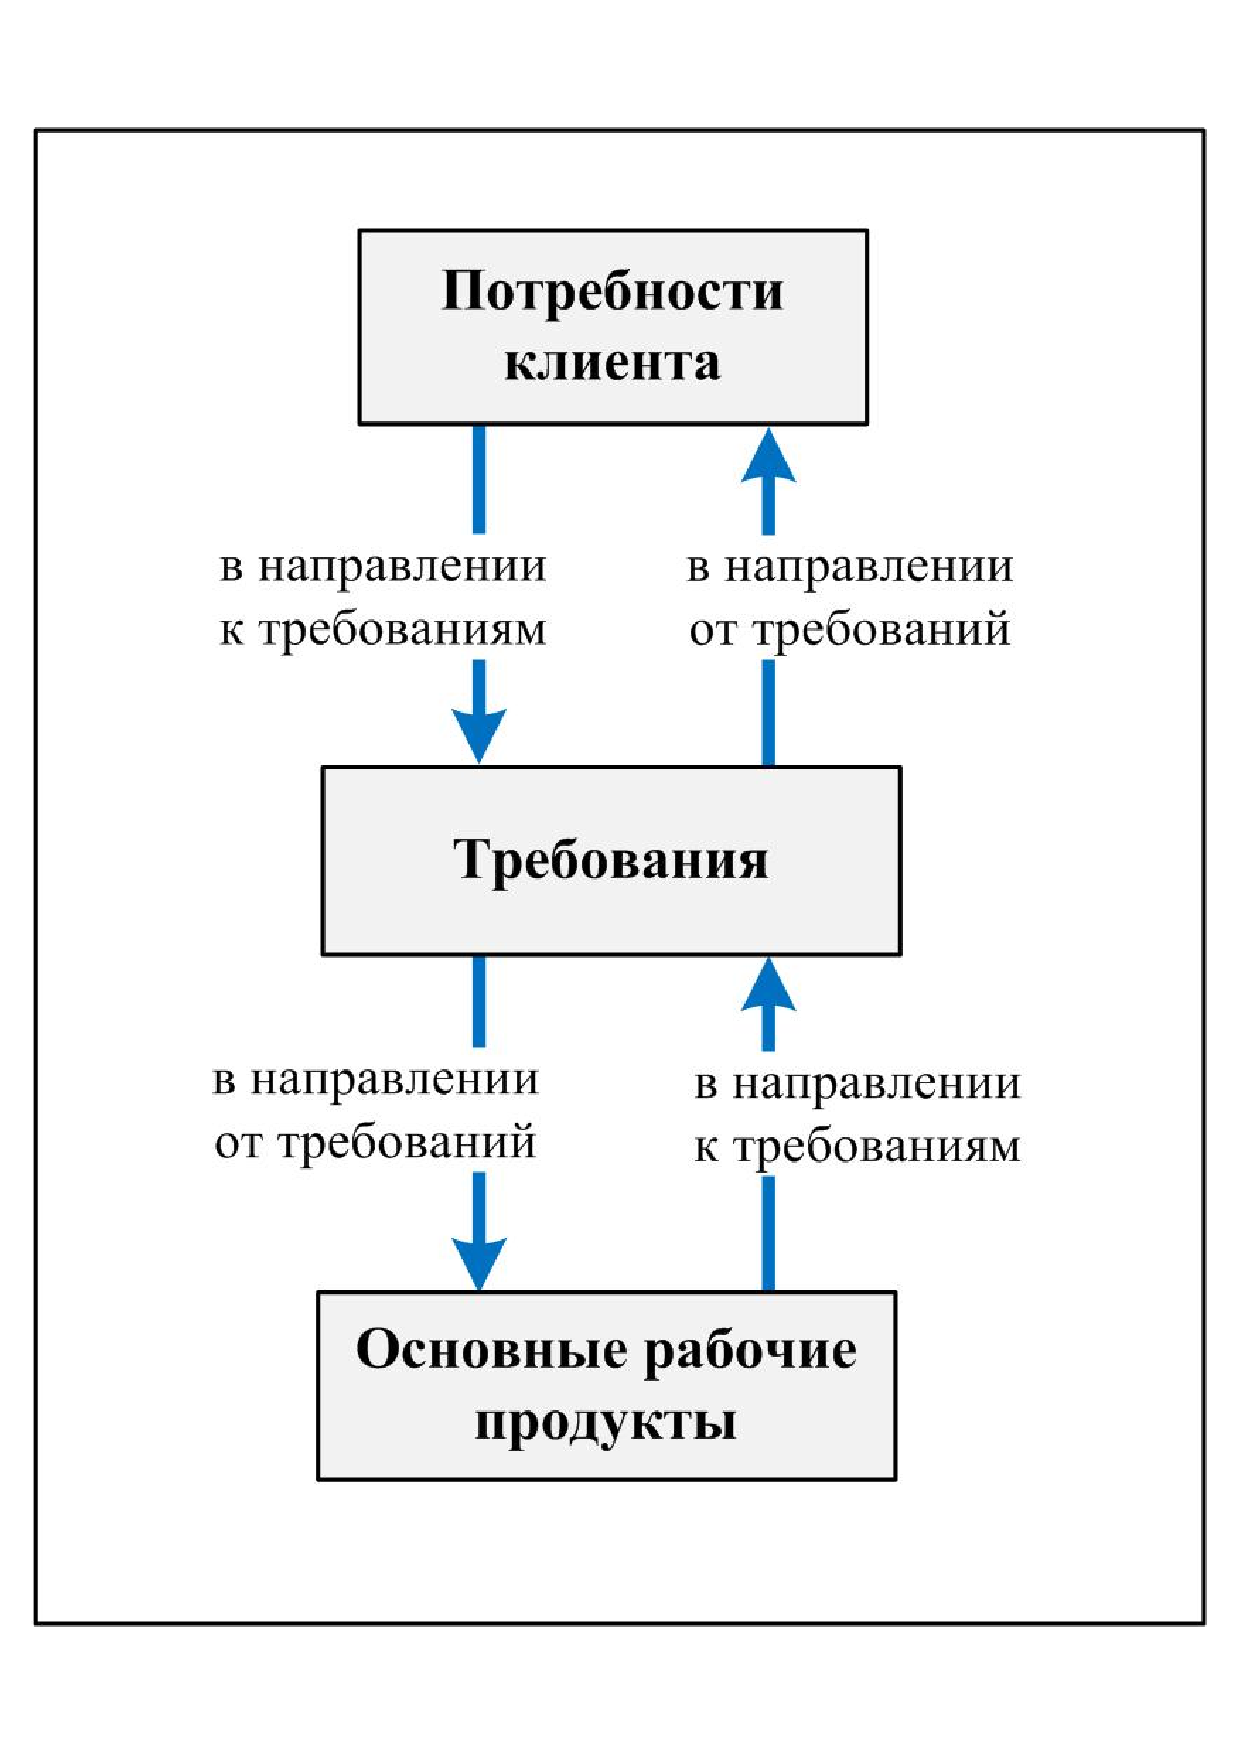
\includegraphics[width=0.5\textwidth]{pic2.pdf}}
\end{frame}

\lecturenotes

На рисунке показаны четыре типа связей отслеживаемости. Потребности клиента отслеживаются в направлении к требованиям, чтобы разработчики смогли определить, которые требования будут затронуты, если в течение или после разработки потребности изменятся. Это также дает уверенность, что в спецификации требований указаны все потребности клиента. И, наоборот, можно проследить направление от требований к потребностям клиента, чтобы определить происхождение каждого требования к ПО

Взглянув на нижнюю часть изображения, можно отслеживать направление от требований, определив связи между отдельными требованиями и элементами продукта. Это тип связи гарантирует, что каждое требование удовлетворено, поскольку разработчику известно, какой компонент соответствует каждому требованию. Четвертый тип связи контролирует отдельные элементы продукта в направлении к требованиям для того, чтобы знать причину созданию каждого элемента~\cite[с.~385--386]{Wiegers}



\section{Инструментальные средства управления требованиями}
\begin{frame} \frametitle{Инструментальные средства управления требованиями}
позволяют пользователям:
	\begin{itemize}
\item импортировать требования из исходных документов
\item определять значения атрибутов, фильтровать
\item выводить на экран содержание базы данных
\item экспортировать требования в различных форматах
\item контролировать связи отслеживаемости
\item соединять требования с элементами, хранящимися в~других средствах разработки ПО
  	\end{itemize}
Важное отличие инструментальных средств "--- способ хранения данных. Все требования, атрибуты и~информация об отслеживаемости хранятся в базе данных
\end{frame}

\lecturenotes

В небольших проектах для управления требованиями, как правило, используются электронные таблицы или простые базы данных, сохраняющие как текст, так и отдельные атрибуты каждого требования. В более крупных проектах выгодно применять коммерческие средства управления требованиями. 

\textbf{Важное отличие инструментальных средств} "--- способ хранения данных. Все требования, атрибуты и информация об отслеживаемости хранятся в базе данных. В зависимости от продукта, база данных может быть коммерческой или разработанной собственными силами и запатентованной, реляционной или объектно-ориентированной. Требования могут импортироваться из различных исходных документов, но затем они сохраняются в базе данных. Как правило, текстовое описание требования считается просто одним из атрибутов. Некоторые продукты позволяют устанавливать связи отдельных требований с внешними файлами (например, файлами Microsoft Word, Microsoft Excel, графическими файлами и т.д.), в которых содержится информация, дополняющая содержимое базы~\cite[с.~400--401]{Wiegers}



\begin{frame} \frametitle{Преимущества использования}
	\begin{itemize}
\item Управление версиями и изменениями (сохранение истории изменений)
\item Хранение атрибутов требований
\item Облегчение анализа воздействия (определение связи между различными требованиями)
\item Отслеживаемость статусов требований (через~отслеживаемость статуса каждого требования)
\item Контролируемый доступ
\item Связь со всеми заинтересованными в проекте лицами (общение с помощью электронных средств обмена информацией)
\item Повторное использование требований (хранение требований в базе данных)
  	\end{itemize}
\end{frame}

\lecturenotes

\textbf{Управление версиями и изменениями.} 
Сам проект должен определять основную версию требований "--- четкий набор требований для конкретной версии. Некоторые средства управления требованиями предлагают функции гибкого управления базовой версией. Они также сохраняют историю изменений каждого требования. Можно записывать обоснование каждого решения об изменении и при необходимости возвращаться к предыдущей версии требования

\textbf{Хранение атрибутов требований.} 
Записывается несколько описательных атрибутов для каждого требования. Каждый, кто работает над проектом, должен иметь доступ к просмотру этих атрибутов, а некоторые — к изменению их значений. Инструментальное средство управления требованиями генерирует несколько системных атрибутов, например дату создания требования и номер его версии, а также, позволяет вам создавать дополнительные атрибуты различных типов данных. Продуманное определение атрибутов позволяет всем заинтересованным в проекте лицам просматривать подмножества требований, основанных на выбранных комбинациях значений атрибутов. Существует возможность запросить список всех требований, основанных на каком-либо бизнес-правиле, чтобы принять решение о последствиях изменения этого правила. Один из способов учета требований в основных версиях различных выпусков продукта "--- использовать атрибут «номер выпуска»

\textbf{Облегчение анализа воздействия.} 
Средства управления требованиями помогают осуществлять отслеживаемость требований, позволяя определять связи между различными типами требований, между требованиями в различных подсистемах и между отдельными требованиями и связанными системными компонентами (например, проектным решением, модулями кода, тестами и пользовательской документацией). Эти связи помогают анализировать воздействие, которое предлагаемое изменение окажет на конкретное требование, выявляя другие элементы системы, которые оно затронет. Другой полезный способ — отследить каждое функциональное требование назад до первоисточника, чтобы знать, откуда оно берет начало

\textbf{Отслеживаемость статусов требований.} 
Собрав требования в базе данных, можно узнать, сколько отдельных требований было указано для продукта. Отслеживаемость статуса каждого требования в процессе разработки способствует общей отслеживаемости статуса проекта. Meнеджер проекта точно представляет себе статус проекта, если знает, что 55\% требований для следующего выпуска проверены, 28\% — реализованы, но не проверены, а 17\% еще не до конца реализованы

\textbf{Контролируемый доступ.} 
Средства управления требованиями позволяют  устанавливать права доступа для отдельных людей и групп пользователей и предоставлять информацию в общий доступ географически распределенной команде через Web-интерфейс к базе данных. Базы данных используют блокировку на уровне требований, позволяя сразу многим пользователям обновлять содержимое базы данных одновременно

\textbf{Связь со всеми заинтересованными в проекте лицами.} 
Некоторые средства управления требованиями позволяют членам команды обсуждать вопросы, связанные с требованиями, на тематических дискуссиях с помощью электронных средств обмена сообщениями. Автоматически отсылаемые электронные сообщения уведомляют членов команды, когда в дискуссии появляется новая запись или любое требование модифицируется. Возможность работы с требованиями через Интернет сокращает расходы на транспорт и уменьшает документооборот

\textbf{Повторное использование требований.} 
Хранение требований в базе данных облегчает их повторное использование в других проектах и подпроектах. Требования, логически подходящие нескольким разделам описания проекта, можно сохранить однажды, а затем лишь ссылаться на них во избежание дублирования требований~\cite[с.~403--404]{Wiegers}.



\begin{frame} \frametitle{Современные инструментальные средства}
	\begin{itemize}
\item IBM Rational DOORS
\item IBM Rational Requisite Pro
\item Borland Caliber DefineIT
\item Borland Caliber RM
\item Compuware Optimal Trace
  	\end{itemize}
\end{frame}

\lecturenotes

	\begin{itemize}
\item IBM Rational DOORS "--- это семейство решений для управления требованиями, которое позволяет оптимизировать обмен информацией о требованиях, контролировать большой объем взаимосвязанной информации, обеспечивает проверку выполнения требований и управление ими. DOORS успешно используется при создании сложных наукоемких изделий (авиа, судостроение, поезда, ракеты, автомобили т.п.)
\item IBM Rational Requisite Pro "--- средство управления требованиями к ПО при разработке программного обеспечения. Оно позволяет разработчикам определять и управлять требованиями, систематизировать и отслеживать изменения, которые могут возникнуть на протяжении всего жизненного цикла проекта, создавать с помощью RationalRequisiteProкачественные сценарии использования, организовывать и повышать эффективность совместной работы
\item Borland Caliber DefineIT предназначен для обеспечения полного и тщательного определения требований с самого начала.
\item Borland Caliber RM "--- корпоративная система управления требованиями, которая разработана для повышения качества создаваемых продуктов, путем улучшения взаимодействия между участниками команды, упрощения анализа влияний требований и процесса передачи информации и возможности непрерывного сбора пожеланий заинтересованных в проекте лиц на всех этапах жизненного цикла проекта
\item Compuware Optimal Trace отображает требования к программному обеспечению с точки зрения пользователя в комплекте с визуальными раскадными досками и отслеживаемыми отношениями на протяжении всего жизненного цикла проекта
  	\end{itemize}




\begin{frame} \frametitle{Функции инструментальных средств}
	\begin{enumerate}
\item Захват/идентификация требований
\item Выделение структуры и организация требований
\item Отслеживаемость требований
\item Управление конфигурациями
\item Формирование отчетов
\item Групповая работа
\item Интерфейсы к другим средствам
\item Системное окружение
\item Пользовательский интерфейс
\item Поддержка
  	\end{enumerate}
\end{frame}


\begin{frame} \frametitle{Функции инструментальных средств}
1. Захват/идентификация требований
	\begin{itemize}
\item Подгрузка внешних документов
\item Автоматический разбор требований
\item Автоматизированная идентификация требований
\item Ручная идентификация требований
\item Пакетные операции
\item Классификация требований
  	\end{itemize}
\end{frame}


\begin{frame} \frametitle{Функции инструментальных средств}
2. Выделение структуры и организация требований
	\begin{itemize}
\item Иерархия требований
\item Различные механизмы представления иерархии
\item Графическое выделение структуры
\item Текстовое выделение структуры требований
\item Ссылки на внешние определения требований (интеграция внешних описаний)
  	\end{itemize}
\end{frame}


\begin{frame} \frametitle{Функции инструментальных средств}
3. Отслеживаемость требований
	\begin{itemize}
\item Выявление противоречий
\item Визуальные ссылки от требований к реализациям
\item Визуальные связь требований и тестовых сценариев
\item Контроль состояния требований
  	\end{itemize}
4. Управление конфигурациями
	\begin{itemize}
\item Ведение истории изменений
\item Использование контроля версий
\item Авторизация на основе групп доступа
  	\end{itemize}
\end{frame}


\begin{frame} \frametitle{Функции инструментальных средств}
5. Формирование отчетов
	\begin{itemize}
\item Поддержка стандартных форматов:MS Word, MS Excel, HTML и др.
		\begin{itemize}
	\item MS Word, MS Excel
	\item HTML 
	\item и др.
  		\end{itemize}
\item Использование проектных словарей
\item Многоязыковая поддержка
\item Настройка отчетов в соответствии с требованиями пользователя
\item Формирование специальных отчетов
  	\end{itemize}
\end{frame}


\begin{frame} \frametitle{Функции инструментальных средств}
6. Групповая работа
	\begin{itemize}
\item Поддержка множественного доступа
\item Многоуровневое назначение прав доступа
\item Встроенный форум для хранения дискуссий о требованиях
\item Возможность offline работы
\item Разрешение конкурентных конфликтов
  	\end{itemize}
\end{frame}


\begin{frame} \frametitle{Функции инструментальных средств}
7. Интерфейсы к другим средствам
	\begin{itemize}
\item Открытые интерфейсы для подключения внешних средств
		\begin{itemize}
	\item Управления проектами
	\item Управления конфигурациями
	\item Управления версиями
  		\end{itemize}
\item Интеграция со средствами:
		\begin{itemize}
	\item Моделирования
	\item Тестирования
	\item Управления проектами
	\item Управления версиями
  		\end{itemize}
\item Импорт данных из стандартных форматов
\item Поддержка XML
  	\end{itemize}
\end{frame}


\begin{frame} \frametitle{Функции инструментальных средств}
8. Системное окружение
	\begin{itemize}
\item Операционные системы
\item Использование коммерческих баз данных
  	\end{itemize}
9. Пользовательский интерфейс
	\begin{itemize}
\item Графический интерфейс
\item WEB-интерфейс
\item Использование скриптов/макросов
  	\end{itemize}
10. Поддержка
	\begin{itemize}
\item Полноценная поддержка
\item Тренинги
\item Демо
\item Документация
  	\end{itemize}
\end{frame}



\begin{frame} \frametitle{Выбор инструментального средства}
	\begin{enumerate}
\item \smallОпределить требования к средству управления требованиями
\item \smallПеречислить 10-15 факторов, которые оказывают влияние на выбор
\item \smallОценить факторы выбора в баллах (всего 100 баллов)
\item \smallСобрать текущую информацию о доступных инструментальных средствах и сравнить их по каждому из~выделенных до этого факторов
\item \smallПодсчитать общую сумму баллов отдельно для каждого инструмента
\item \smallПопросить других пользователей составить отчеты об~использовании каждого продукта
\item \smallПопросить производителей прислать для оценки инструментальные средства, занявшие верхние места в~получившемся рейтинге
\item \smallОценить инструментальные средства, применяя их в~реальном проекте
\item \smallПринять решение
  	\end{enumerate}
\end{frame}


\lecturenotes

Некоторые компании нанимают для оценки инструментальных средств консультантов, которые могут оценить все нужды компании и порекомендовать доступный продукт. Если оценка проводится самостоятельно, то рекомендуется придерживаться следующих рекомендаций:
	\begin{enumerate}
\item Определить требования организации к средству управления требованиями. Установить, какие возможности наиболее существенны, с какими еще средствами хотелось бы интегрировать продукт, насколько важен удаленный доступ к данным через Интернет. Решить "--- использовать для хранения некоторой информации о требованиях текстовые документы или предпочесть базу данных
\item Перечислить 10-15 факторов, которые оказывают влияние на выбор. Учесть такие субъективные категории, как возможности индивидуальной настройки, эффективность продукта и интерфейса пользователя. Стоимость, конечно же, важна, но прежде оцениваются сами инструментальные средства
\item Оценить факторы выбора, перечисленные в пункте 2, в баллах (всего 100 баллов), назначая большее значение тем факторам, которые являются для организации более важными
\item Собрать текущую информацию о доступных инструментальных средствах управления требованиями и сравнить их по каждому из выделенных до этого факторов. С оценкой субъективных факторов придется подождать до тех пор, пока не представится возможность непосредственно поработать с каждым средством. Демонстрация продукта производителем может прояснить некоторые вещи, но скорее всего, будут показаны наиболее сильные стороны инструмента. Демонстрация не заменит самостоятельную работу с продуктом в течение нескольких часов
\item Подсчитать общую сумму отдельно для каждого инструмента, сложив баллы, которые были определены для каждого пункта, уже после чего будет ясно, какие продукты подходят лучше всего.
\item Попросить других пользователей составить отчеты об использовании каждого продукта, например, разместив запросы на форумах в Интернете, чтобы дополнить вашу собственную оценку, а также запросить у поставщика литературу, демо-версию продукта и данные о цене
\item Попросить производителей прислать для оценки инструментальные средства, занявшие верхние места в получившемся рейтинге. Определить, как будет проводиться оценка до установки их на компьютер, чтобы быть уверенным, что необходимая информация для принятия решения будет получена
\item Оценить инструментальные средства, применяя их в реальном проекте, а не только в обучающем проекте, поставляемом с продуктом. Завершив оценку, при необходимости уточнить параметры оценки и выяснить, какой из продуктов теперь лидирует
\item Принять решение, учитывая как количество очков, набранных каждым продуктом, стоимость лицензий и расходов на сопровождение, так и мнение других пользователей и субъективные впечатления членов команды от каждого продукта~\cite[с.~408--409]{Wiegers}
  	\end{enumerate}



\begin{thebibliography}{99}
\bibitem{Wiegers} Вигерс Карл, Разработка требований к программному обеспечению / Пер, с англ. "--- М.: Издательсш-торговый дом «Русская Редакция», 2004. "--- 575с.: ил.
\bibitem{Maglinec} \href{http://ivan-shamaev.ru/wp-content/uploads/2013/06/Information-systems-analysis-and-requirements-analysis.pdf}{Анализ требований к информационным системам. Учебное пособие, Маглинец Ю.А., 2007}
\end{thebibliography}

\end{document}

%%% Local Variables: 
%%% mode: TeX-pdf
%%% TeX-master: t
%%% End: 
